%
% General structure for the revdetua class:
%
\documentclass[english]{revdetua}
%
% Valid options are:
%
%   longpaper --------- \part and \tableofcontents defined
%   shortpaper -------- \part and \tableofcontents not defined (default)
%
%   english ----------- main language is English (default)
%   portugues --------- main language is Portuguese
%
%   draft ------------- draft version
%   final ------------- final version (default)
%
%   times ------------- use times (postscript) fonts for text
%
%   mirror ------------ prints a mirror image of the paper (with dvips)
%
%   visiblelabels ----- \SL, \SN, \SP, \EL, \EN, etc. defined
%   invisiblelabels --- \SL, \SN, \SP, \EL, \EN, etc. not defined (default)
%
% Note: the final version should use the times fonts
% Note: the really final version should also use the mirror option
%
\usepackage{graphicx} 
\usepackage{listings} %code highlighter
\usepackage{color} %use color
\definecolor{lightgray}{rgb}{.9,.9,.9}
\definecolor{darkgray}{rgb}{.4,.4,.4}
\definecolor{purple}{rgb}{0.65, 0.12, 0.82}
\lstdefinelanguage{JavaScript}{
  keywords={break, case, catch, continue, debugger, default, delete, do, else, false, finally, for, function, if, in, instanceof, new, null, return, switch, this, throw, true, try, typeof, var, void, while, with},
  morecomment=[l]{//},
  morecomment=[s]{/*}{*/},
  morestring=[b]',
  morestring=[b]",
  ndkeywords={class, export, boolean, throw, implements, import, this},
  keywordstyle=\color{blue}\bfseries,
  ndkeywordstyle=\color{darkgray}\bfseries,
  identifierstyle=\color{black},
  commentstyle=\color{purple}\ttfamily,
  stringstyle=\color{red}\ttfamily,
  sensitive=true
}

\lstset{
   language=JavaScript,
   backgroundcolor=\color{white},
   extendedchars=true,
   basicstyle=\footnotesize\ttfamily,
   showstringspaces=false,
   showspaces=false,
   tabsize=2,
   breaklines=true,
   showtabs=false,
   captionpos=b
}

\begin{document}

\Header{1}{1}{Novembro}{2019}{1}
% Note: the month must be in Portuguese

\title{WebGL Racing Car Game}
\author{Xavier Santos \and Daniel Carvalho} % or \author{... \and ...}
\maketitle

\begin{abstract}
  A simple arcade-like racing car game running in WebGL/JavaScript for the first project in the Computação Visual course.
\end{abstract}

\section{Game context and rules}
The game consists of the player's car evading obstacles \textit{ad infinitum} until it is hit.
\\
To start the game the player should load the model of the car from \textbf{models/car.obj} and then press the \textit{space key} to start playing.
\\
The rules are the following:

\begin{itemize}
	\item The player's car moves countinously forward and the player may alternate between three lanes.
	\item There will appear obstacles from which the player must dodge by changing lanes.
	\item The car's speed increases as the game goes by capping at a limit.
	\item The score increases acoording to the distance travelled by the vehicle.
	\item The game ends when the player's car collides with an obstacle.
\end{itemize}

The score and speed of the car are displayed in the page, as well as the \textit{FPS}.

\section{Canvas}
To display the models we use a 600x448 WebGL canvas with an image background and set the default scaling of the X coordinate to 600/448 to keep the aspect ratio of the models in a wider display.

\begin{figure}[h]
	\centering
	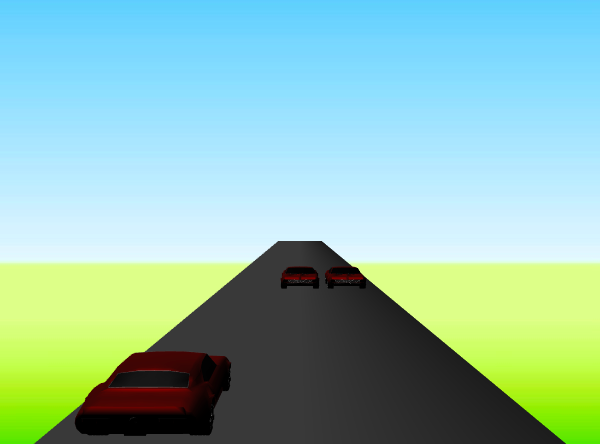
\includegraphics[width=\linewidth]{game.png}  
	\caption{Game canvas}
	\label{fig:game}
\end{figure}

\section{Camera}
The view volume is set in prespective mode with the user at the point (0,0,0) with a 45 degree FoV and a view distance of 30. To give a sense of depth and to percieve the distance of the incoming obstacles.

\begin{lstlisting}[language=JavaScript]
	pMatrix = perspective( 45, 1, 0.05, 30 );
\end{lstlisting}

The models move between Z=-30 and Z=1. The \textit{near} field of the prespective matrix is set to 0.05 and the whole scene is moved -2.5 on the Z axis.

\section{Game models}
There are two different simple mesh models in the game. One is the road, which has a single face composed by two triangles and scaled up on the Z axis to generate a long rectangle in the XoZ plane. The other ones are simple cubes. These are only placeholders and will be replaced by the car model once the user inputs the OBJ file, which is then read by a function adapted from the obj-reader used in class. The car model was downloaded from \url{free3d.com} and then edited and simplified using MeshLab\footnote{\url{www.meshlab.net}} to create an OBJ file with the information of the vertex, vertex normals, vertex colors and faces of the 3D model.

\begin{figure}[h]
	\centering
	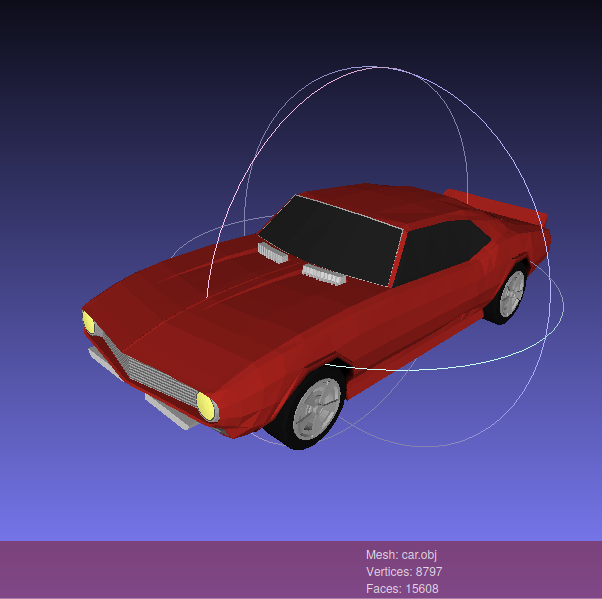
\includegraphics[width=\linewidth]{car_meshlab.png}  
	\caption{3D car model in MeshLab}
	\label{fig:car_meshlab}
\end{figure}

\section{Ligh Sources}
The scene features two sources of light. A static one coming from above and slightly behind the player's vehicle and another rotating around the scene on the X and Y axis. As the colors are mainly given by the vertex's uniform color, the light sources are white to preserve that color and just add a reflection effect on the models.

\begin{lstlisting}[language=JavaScript]
	var lightSources = [];

	// Light source 0

	lightSources.push(new LightSource());

	lightSources[0].setPosition(-2.0,2.0,0.0,0.0);

	lightSources[0].setIntensity(1.0,1.0,1.0);

	lightSources[0].setAmbIntensity(0.2,0.2,0.2);

	lightSources[0].switchRotYYOn();

	lightSources[0].switchRotXXOn();

	lightSources[0].setRotationSpeed(1.0);

	// Light source 1

	lightSources.push(new LightSource());

	lightSources[1].setPosition(0.0,10.0,1.0,0.0);

	lightSources[1].setIntensity(0.8,0.8,0.8);

	lightSources[1].setAmbIntensity(0.5,0.5,0.5);
\end{lstlisting}

\section{Colors}
To obtain the colors of the models, first we obtain the color resulting from the ilumination according to Phong's model and then we multiply it with the vertex color, which is given directly to the model, either by the OBJ file or directly to the vertices in the sceneModels constructor.

\begin{lstlisting}[language=JavaScript]
	//shader-vs
	fColor += diffuse + specular;	
	vertexColor = vec4(aVertexColor, 1.0);

	//shader-fs	
	void main(void) {
		gl_FragColor = fColor * vertexColor;
	}
\end{lstlisting}

\section{Animation}
Game logic and animation are mainly implemented in the \textbf{game\textunderscore functions.js} file. The \textbf{gameStart()} function is triggered by pressing the \textit{space key}, this function sets the position of the obstacles to Z=-30, the intitial speed of the game is set/reset as well as the score.
\\
When the game is runnig it is controlled by the \textbf{obstaclesMove(speed)} function. There is applied a translaction to the objects positively across the Z axis according to the current speed of the game. If the obstacles are in the same Z position as the player, there will be a check for a collision. In the case there is a collision the game will stop an the player's vehicle will start rotating around the Y axis. Having no collisions, the obstacles will reach the end of the view space and respawn in a random lane back at Z=-30 and the game speed will increase if the speed limit has not yet been reached.

\begin{lstlisting}[language=JavaScript]
	function obstaclesMove ( speed ) {
		obstacle1.tz = obstacle2.tz += speed

		if (obstacle1.tz >= 0 || obstacle2.tz >= 0) {
			checkColision();
		}

		if (obstacle1.tz >= 1 || obstacle2.tz >= 1){
			resetObstacles();
			if(gameSpeed < 0.50){
				gameSpeed += 0.01;
				carSpeed = Math.floor(gameSpeed * 1000 - 100);
				document.getElementById('car_speed').innerHTML = 'SPEED: ' + carSpeed + ' KPH';
				score += gameSpeed * 1000;
				document.getElementById('score').innerHTML = 'SCORE: ' + score;
			}
		}
	}
\end{lstlisting}

\section{Conclusion}
The game is fully functional and running without noticeable bugs in vanilla JavaScript and WebGL using the code provided by the professor in the practical classes. The view angle selection was not implemented as it was not a relevant feature for the gameplay.
\\
There was an effort to include textures in the road but as this feature was not totally implemented it was left out of the final release. Although, some residual code for the texture implementation was left commented in the shaders and the main JavaScript code.

\end{document}